\subsection{Steered Response Power}

Steered Response Power (SRP) source localization is a method to detect sound source locations using beamforming techniques \cite{krim1996two}. SRP is different from TDOA based methods discussed before. While the generalized cross correlation is a simple cross correlation between each pair of microphones and only outputs an estimate of the time delay, the SRP method beamforms the space around the array and computes the energy of each location beam.  It `looks' at all possible directions individually (steering) and computes the power of the signal cross correlation in that direction (beamforming). The assumption is that the cross power of the steered microphone array will be the maximum in the correct source direction. However, the computational demand for this can rise quite fast (depending on the sampling rate and the angular resolution of the beamforming), making it nearly impossible to implement in real time applications. However, its performance in difficult conditions outperforms the TDOA based methods \cite{dmochowski2007generalized}. Since real-time localization is not of primary importance for this thesis, SRP based methods can be applied. In the same fashion as the GCC method proposed to pre-filter the signal before performing the cross correlation, a PHAT weighing can be applied on the beamformed signal. This method is called SRP-PHAT. In this section, the first part discusses the basic principles behind the method whereas the second part introduces a hybrid method that improves the computational time of SRP without decreasing its robustness. 

%\subsubsection{Steered Beamformer}

The SRP method is based on a regular delay-and-sum beamformer, for a given point in space having range $\rho$, azimuth $\theta$ and elevation $\phi$ with the microphone array, the output of the beamformer is given by

\begin{equation}
    y_{\rho,\theta,\phi}(n)=\sum\limits_{m=0}^{M-1}{w_m x_m[n + f_{0,m}(\rho,\theta,\phi)]},
\end{equation}

where $x_0[n]$ is the signal received at time n, at an arbitrary microphone used as reference, $w_m$ is the amplitude weight for microphone m, and $f_{0,m}(\rho,\theta,\phi)$ is the relative delay between the reference microphone and the $m^{th}$ microphone. When far-field approximation is assumed, the range cannot be computed and the delay-and-sum beamformer output can be rewritten as follows:

\begin{equation}
    y_{\theta,\phi}(n)=\sum\limits_{m=0}^{M-1}{w_m x_m[n + f_{0,m}(\theta,\phi)]} 
\end{equation}


For $w_m=1$ (assuming perfectly omni-directional and equally sensitive microphones), the output power of the beamformer becomes

\begin{equation}
    \mathbb{E}[{y_{\theta,\phi}(n)^2}]=\sum\limits_{i=0}^{M-1}\sum\limits_{j=0}^{M-1}{R_{x_i,x_j}[f_{i,j}(\theta,\phi)]} 
    \label{eq:poweroutputbeamformer}
\end{equation}

This cross correlation is computed in the frequency domain using cross-spectrum which is then inverse fast Fourier transformed (IFFT).

\begin{equation}
    R_{x_i,x_j}(\tau)= \sum\limits_{k=0}^{N_{f}-1}{X_{i}(k)X_{j}^*(k)e^{j2\pi\frac{k}{N_{f}}\tau}}
\end{equation}

%\subsubsection{SRP Search}

The SRP method starts with a look up procedure which associates each set of angles ($\phi,\theta$) to a given set of delays between each microphone pair. For instance if we use a 1$\degree$  resolution, the SRP method associates 360*360=129600 angular positions to corresponding delays. The cross correlations of the signals received at the different microphone pairs combinations possible are then computed. For a given position ($\phi,\theta$), the output of the SRP search is simply the sum of the cross correlation at each time delay found relative to each pair of microphone. It corresponds to the power output of the beamformer defined in Eq. \ref{eq:poweroutputbeamformer}. 
\begin{equation}
    S_{SRP}(\theta,\phi)=\sum\limits_{i=0}^{M-1}\sum\limits_{j=0}^{M-1}{R_{x_i,x_j}[f_{i,j}(\theta,\phi)]}
     \label{eq:srpSum}
\end{equation}

\begin{figure}[H]
    \centering
    \begin{subfigure}[t]{0.5\textwidth}
    \centering
    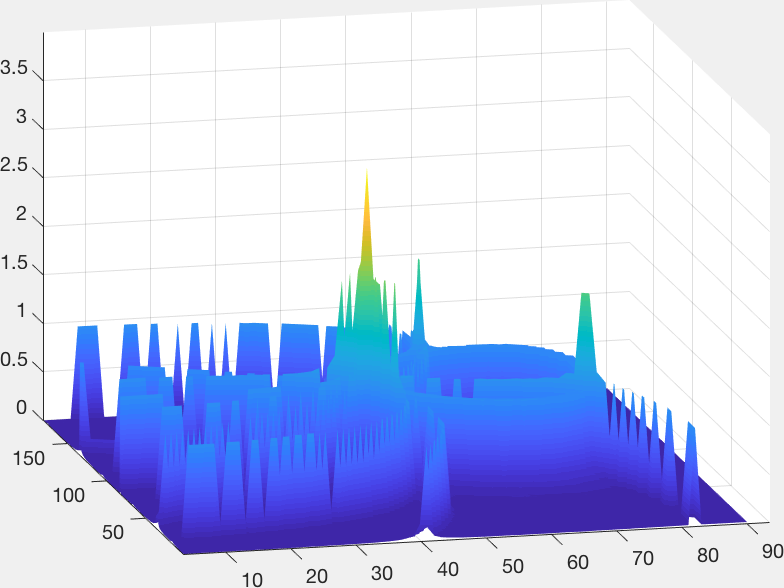
\includegraphics[width=0.9\textwidth]{Figures/viewside.png}
    \caption{SRP map}
    \label{fig:viewsidesrp}
\end{subfigure}%
\begin{subfigure}[t]{0.5\textwidth}
    \centering
    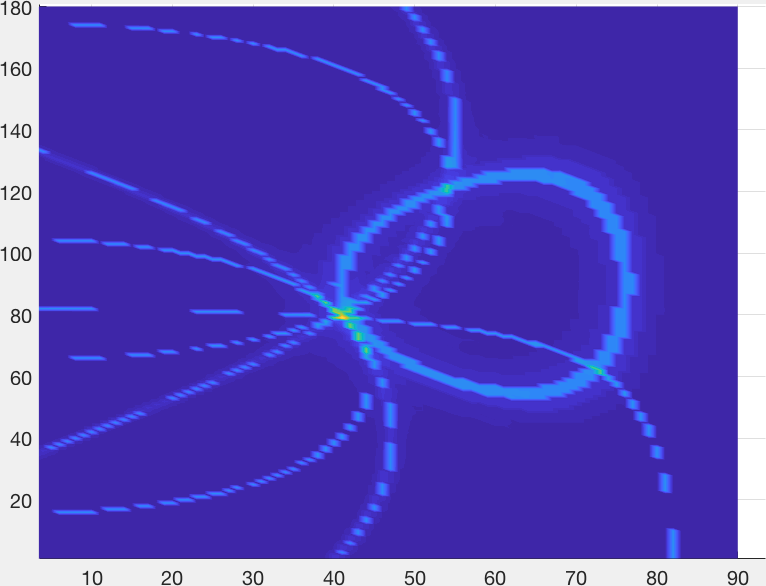
\includegraphics[width=0.9\textwidth]{Figures/topview.png}
    \caption{SRP heat map}
    \label{fig:topviewsrp}
\end{subfigure}
\caption{Power mapping simulation of source localized using SRP-PHAT algorithm in noiseless, free-field situation. For the simulation, first a 4-channel wav file is created such that the channels contain the same pink noise but delayed between each other. The delays are such that the source would be ideally located at azimuth $80\degree$ and elevation $40\degree$ when localized by a 1m aperture tetrahedral array. SRP-PHAT is then applied on the wav file and power received from different angles (beams) is computed and plotted. As can be seen the algorithm was able to localize the source in these ideal conditions fairly correctly.}
\end{figure}

The SRP method estimates the source location ($\hat{\phi},\hat{\theta}$) after creating the SRP search space such that

\begin{equation}
    \hat{\phi},\hat{\theta}=\argmax_{\phi,\theta}S_{SRP}(\phi,\theta)
\end{equation}

%\subsubsection{Premapping the delays to potential sources locations}

The classical SRP search beamforms sequentially the 3D space and locations [($\phi_{1},\theta_{1}$), ($\phi_{2},\theta_{2}$), ... ,($\phi_{x},\theta_{x}$)] which might be associated with the same relative delay $\tau_{1}$ (in case of a uniform linear microphone array). The cross correlation at delay $\tau_{1}$ is then computed $x$ times, which leads to the same results for each [($\phi_{1},\theta_{1}$), ($\phi_{2},\theta_{2}$), ... ,($\phi_{x},\theta_{x}$)] positions, leading to numerous useless cross correlation computations. In \cite{dmochowski2007generalized} the authors propose an improvement on the SRP search algorithm by pre-mapping the relative delays to their corresponding set of locations. Instead of proceeding to a sequential search in the 3D space, a search on the possible relative delays is considered. The possible delays between individual microphone pairs are already known based on the array geometry and can be stored in memory. The cross correlations are calculated for each delay subset and related to a set of potential source location in space in the final steps of the algorithm. Note that the computational cost gain can be immense depending on the number of microphones (the more the microphones, the greater the gain), the aperture size (the smaller the microphone array the more angles are associated with the same time delay) or the sampling rate (again the smaller the sampling rate the more angles are associated with the same time delay). In GCC methods this issue was taken care of by interpolation, where the microphone pair end-side localization had poor resolution (Fig. \ref{fig:res_diff}). 

The method can be easily extended to SRP-PHAT, where pre-filtering the signal beforehand by using PHAT introduces a function $\psi_{ij}$ in the cross correlation

\begin{equation}
    R_{x_i,x_j}(\tau)= \sum\limits_{k=0}^{N_{f}-1}{\psi_{ij}(k) X_{i}(k)X_{j}^*(k)e^{j2\pi\frac{k}{N_{f}}\tau}}
\end{equation}
where
\begin{equation}
    \psi_{ij}(k) = \frac{1}{|{X_{i}(k)X_{j}^*(k)}|}
\end{equation}

%\subsubsection{Simulations}

%Two identical sound sources are placed in the far field. A tetrahedral array with equal spacing between microphones of 1 meter is receiving the two sources. The sound received at the sources are 3 seconds of two different pink noises with respective DOA $\tetha_{1}=120\degree$, $\phi_{1}=40\degree $ and $\tetha_{2}=150\degree $ , $\phi_{2}=75\degree $. Waves are propagating in free field where no reflections and no noise is added to the microphones. The SRP maps are computed and displayed in the figure \ref{fig:coherent2pinknoise}. Source 2 is placed at a problematic angle for the tetrahedral array, detection errors are discussed in section \ref{sec:detection}. Error probability increases as the source DOA approach the angle of the axis drawn by pairs of microphones (end-side).

%\begin{figure}[H]
%    \centering
%    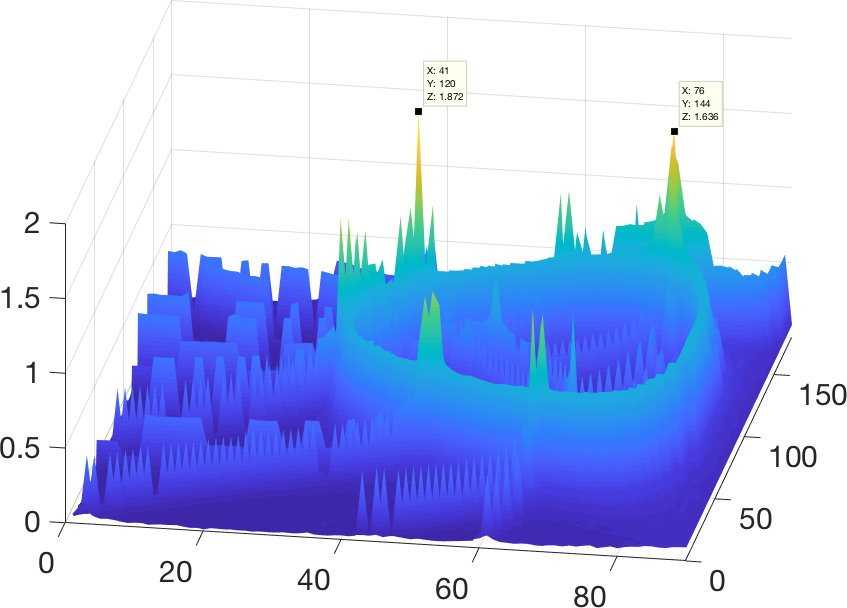
\includegraphics[width=1\textwidth]{Figures/2pinknoisesrpphat.png}
%    \caption{SRP-PHAT simulation with 2 sound sources localized using a tetrahedral array}
%    \label{fig:coherent2pinknoise}
%\end{figure}



%\subsubsection{Localization errors} \label{sec:detection}

%Two pairs of microphones are considered, the axes drawn by the two pairs is plotted (extended) in figure \ref{fig:locerrortetra}. The two axes form respective angles of $45\degree$ and $60\degree$ with the horizontal axis. Plane waves with DOA between $45\degree$ and $60\degree$ will cross the two pairs of microphones at an angle close to the respective end-sides of the pairs. As shown in figure \ref{fig:errorsimulation1} maximum errors arise in the simulation for DOA contained in between $45\degree$ and $60\degree$. For a tetrahedral array, this can be seen as the 3d space created by extending the arms connecting the microphones. 

%\begin{figure}[H]
%    \centering
%    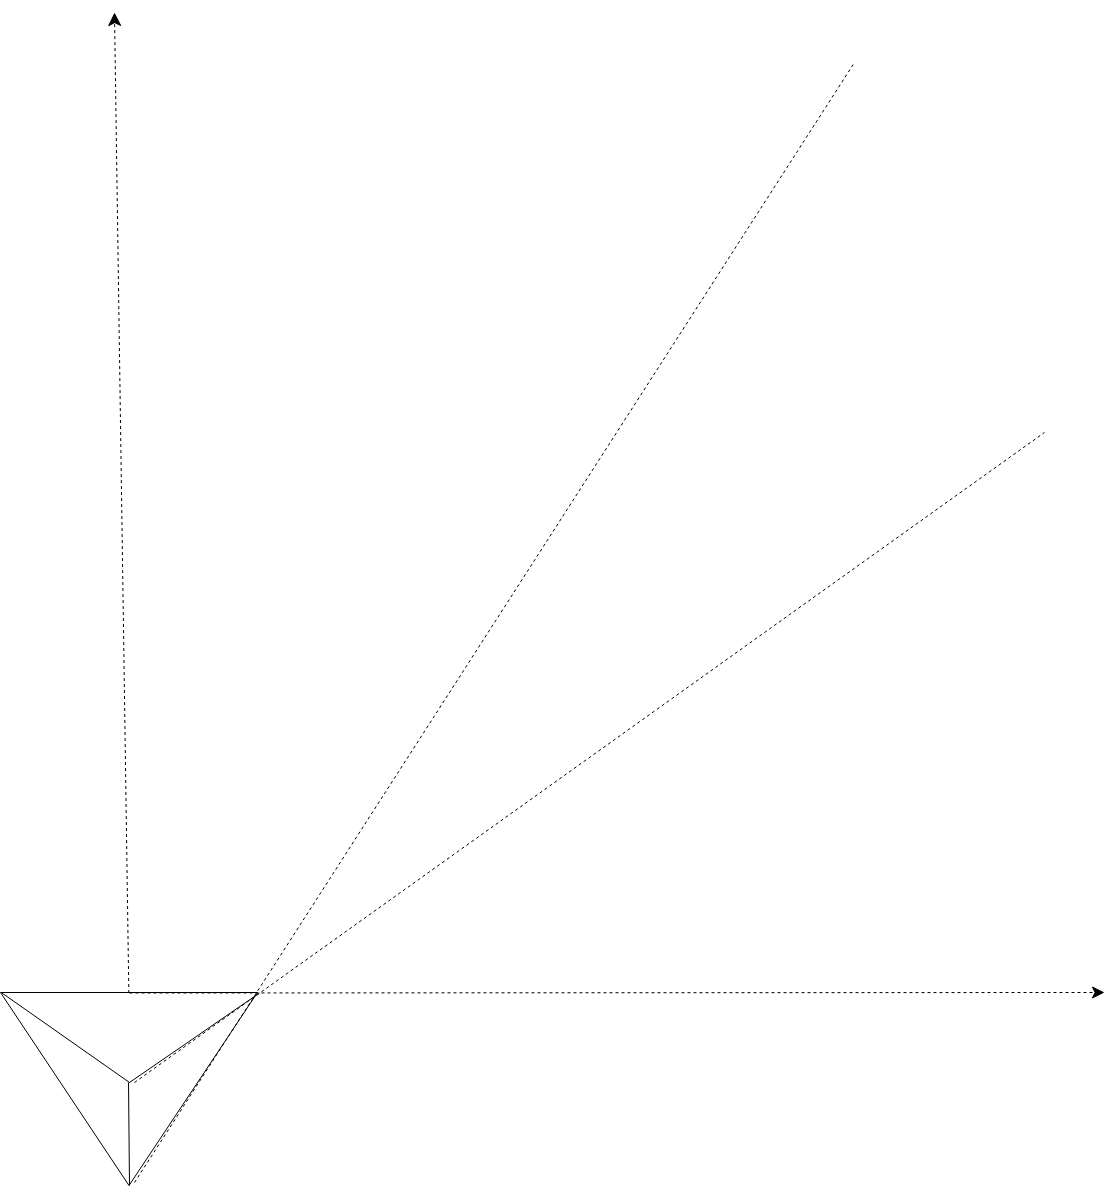
\includegraphics[width=0.9\textwidth]{Figures/locerrors.png}
%    \caption{Axis drawn by 2 pairs of microphones}
%    \label{fig:locerrortetra}
%\end{figure}

%\begin{figure}[H]
%    \centering
%    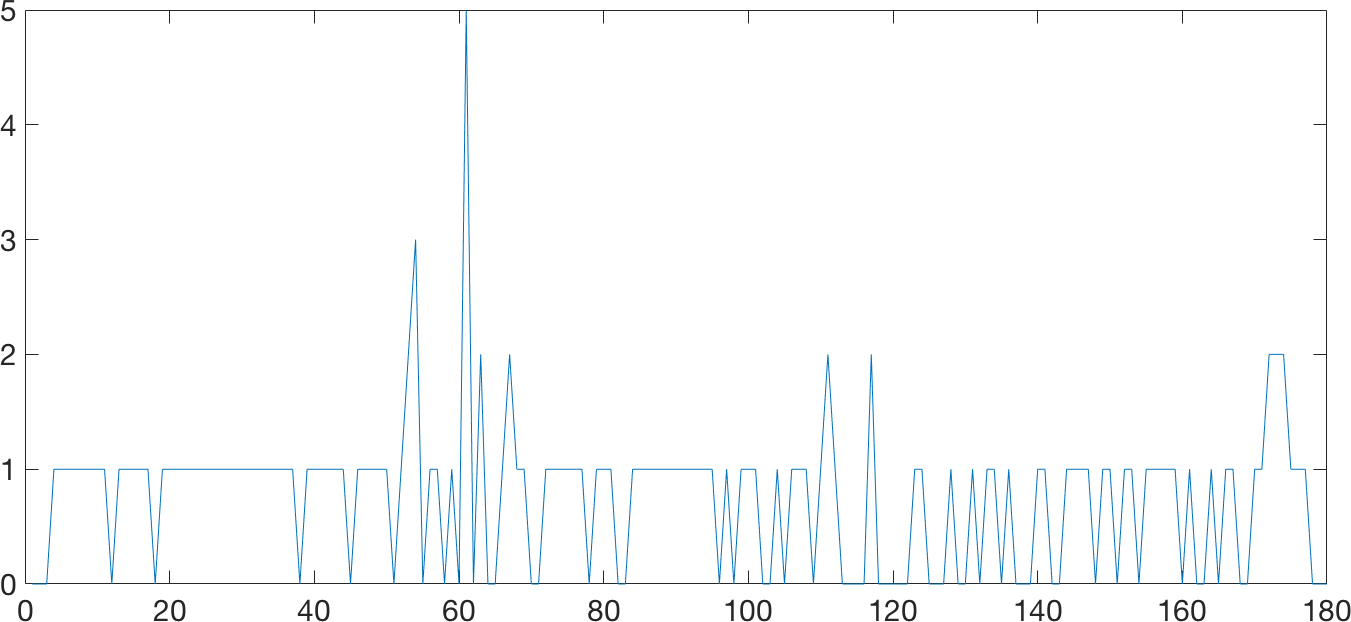
\includegraphics[width=0.9\textwidth]{Figures/errorphinointerpolationandrounding.png}
%    \caption{Simulation errors with no interpolation}
%    \label{fig:errorsimulation1}
%\end{figure}

%\subsubsection{Temperature and noise}

%Temperature is a major parameter of the algorithm and it affects the speed of sound in air and ultimately the propagation delay in the array.



%\subsubsection{SRP vs SRP PHAT}

%An experiment is design to test our implementations of SRP and SRP PHAT. A prototype tetrahedral microphone array is placed outside, the ideal free field condition are not holding since ground effect and reflections from the nearby buildings will affect the sound waves received by the array. The SNR cannot be controlled and is found to be, 

